\subsection{Рекуррентные нейронные сети (RNN)}
В случае сверточных нейронных сетей, текст позиционировался как пространственная структура. 
В случае рекуррентных нейронных сетей \cite{Schmidhuber2015, Schmidhuber:1996} следует рассматривать его как последовательность,
информация об элементе которой находится в зависимости от предшествующих ему элементов, 
другими словами, текст имеет направленное повествование. 
Подобная структура присуща не только текстам, но также и аудиосигналам или временным рядам.  
\subsubsection{Традиционные RNN}
Основная идея рекуррентных нейронных сетей зиждется на введении скрытых состояний 
и определении новых состояний через предыдущие. Таким образом, происходит латентное запоминание информации.
 То есть, в отличие от других нейронных сетей (сверточных, полносвязных), рекуррентная определяет своё состояние 
 не только за счет входных данных, но и за счет предыдущих состояний.
 \begin{figure}[ht]
     \centering
     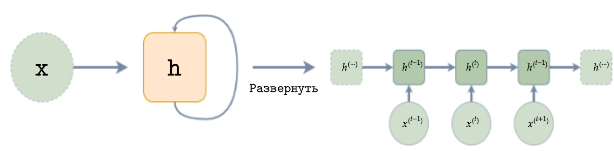
\includegraphics[scale=2]{rnn1}
     \label{rnn1}
     \caption{Развернутая рекуррентная нейронная сеть без выходов}
 \end{figure}
 
 На каждом шаге рекуррентной сети:
 \begin{enumerate}
     \item Прочитать очередной элемент последовательности $x^{t}$,
      применить к нему линейное преобразование:
      \[z^{t} = W_{\text{input}} \cdot x^t;\]
     \item Вычислить новое значение состояния, исходя из старого:
      \[h^{t} = \mathrm{act} \left(W_{\text{hidden}} \cdot h^{t-1} + z^{t}\right);\]
     \item Выйти из рекуррентного шага:
      \[y^{t} = W_{\text{output}} \cdot h^{t}.\]
 \end{enumerate}

 \bigskip\par
 Обучаемыми параметрами являются веса $W_{\text{input}}, W_{\text{hidden}}, W_{\text{output}}$, участвующие в линейных преобразованиях.
Нулевое состояние сети может задаваться различными способами: исходя из экспериментальных показателей, лучше всего использовать малодисперсный шум \cite{Goodfellow}.

\bigskip\par
Основными проблемами рекуррентных нейронных сетей во время обучения являются сходимости: возникают взрыв и затухание градиента. Рассмотрим эти ситуации подробнее.
\subsubsection{Затухание и взрыв градиента}
Рассмотрим прямой проход (forward pass) по классической рекуррентной нейронной сети (Vanilla RNN) на рис. \ref{fig:rnn3} 
\begin{figure}[ht]
    \centering
    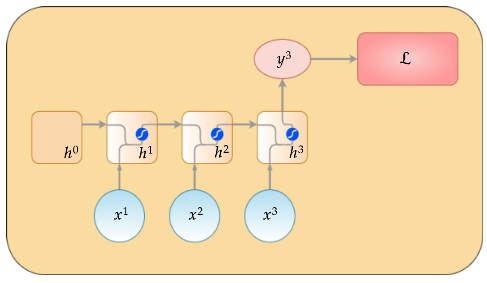
\includegraphics[scale=1.5]{rnn3.png}
    \caption{Vanilla RNN}
    \label{fig:rnn3}
\end{figure}

Введем обозначения. Входная последовательность $x^{t} \in \mathbb{R}$, скрытое состояние $h^{t} = f(w\cdot h^{t-1} + x^{t}),$ где $f$ -- нелинейная, дифференцируемая функция активации, $w \in \mathbb{R}$ -- параметр функции перехода, $y^{t} = g(h^{t})$ -- выход, функция потерь (функция ошибки, функционал качества) $\mathcal{L}(y^{t})$:
\begin{enumerate}
    \item $h^{0} \in \mathbb{R}$;
    \item $h^{1} = f(w\cdot h^{0} + x^1)$;
    \item $h^{2} = f(w\cdot h^{1} + x^{2}) = f\left(w \cdot f \left(w \cdot h^{1} + x^{2}\right) + x^{3}\right) = \\\hspace{0.5cm}=f\left(w \cdot f\left(w \cdot f\left(w \cdot h^{0} + x^{1}\right) + x^{2}\right) + x^{3}\right).$
\end{enumerate}
Выполним обратный проход (back propogation through time \cite{Zipser:1}):
\begin{gather*}
\mathcal{L} (y^{3}) = \mathcal{L} \left(g\left(h^{3}\right)\right) = \mathcal{L}\left(g\left(f\left(w\cdot h^{2} + x^{3}\right)\right)\right) = \\ = \mathcal{L}\left(g\left(f\left(w\cdot f\left(w\cdot h^{1} + x^{2}\right) + x^{3}\right)\right)\right)    
\end{gather*}
Применяя градиентный спуск, нам понадобится производная по параметрам:
\[\frac{\partial \mathcal{L}\left(y^{3}\right)}{\partial w} = \frac{\partial \mathcal{L}\left(y^{3}\right)}{\partial g}\cdot \frac{\partial g}{\partial w} = \frac{\partial \mathcal{}{L}\left(y^{3}\right)}{\partial g} \cdot \frac{\partial g}{\partial f}\cdot \frac{\partial f\left(w\cdot h^{2} + x^{3}\right)}{\partial w}\]
\begin{gather*}
    \frac{\partial f\left(w\cdot h^{2} + x^{3}\right)}{\partial w} = f'\left(w\cdot h^{2}+ x^{3}\right)\cdot \left(w\cdot h^{2} + x^{3}\right)' = f_{3}'\cdot \left(w \cdot h^{2}\right)' = \\ = f_{3}'\left(w'\cdot h^{2} + w \cdot h^{2'}\right) - f_{3}'\cdot \left(h^{2} + w\cdot f\left(w \cdot h^{1} + x^{2}\right)'\right) = \\ = f_{3}'\cdot \left(h^{2}+ w\cdot f_{2}' \cdot \left(h^{1} + w\cdot f\left(w\cdot h^{0}+ x^{1}\right)'\right)\right) = \\ = \sum\limits_{i = 1}^{3} \left(h^{i-1} \cdot w^{3-i}\prod\limits_{j=i}^{3}f_{j}'\right)
\end{gather*}
Именно последнее умножение является причиной затухания или взрыва градиента. Одной из часто употребляемых функций активаций является гиперболический тангенс, производная которого лежит в диапазоне: $0 < \tanh' < 1$.
Умножение большого числа таких значений приведет к затуханию градиента (vanishing gradient) \cite{Zipser:1}. Борьбой с этим является ограничение количества скрытых состояний, что, по сути, ограничивает обрабатываемые последовательности. Основная идея рекуррентных нейронных сетей теряет смысл при подобном решении проблемы.

\bigskip\par
С другой стороны, если модуль произведения больше единицы, то произойдет взрыв градиента, приводящий к переполнению и падению точности. Борьба с такой проблемой является более очевидной -- ограничение на сам градиент (ввод фиксированной величины, превышение которой ограничивает превысивший ее градиент этой величиной). 

\bigskip\par
Затухающий градент так же связан с долгосрочными зависимостями \cite{Schmidhuber2001}. Любые флуктуации в краткосрочных зависимостях буду подавлять долгосрочные. В случае, если модель способна представить долгосрочные зависимости, градиент долгосрочного взаимодействия будет экспоненциально ниже краткосрочного \cite{Goodfellow}.

\bigskip\par
В связи с таким поведением градиента при обучении возникает явная проблема борьбы между мощностью и обучаемостью рекуррентных сетей. Ради ее решения были разработаны специализированные архитектуры рекуррентных нейронных сетей: LSTM \cite{Schmidhuber:1996} и GRU \cite{Sutskever:1}.
\subsubsection{Долгая краткосрочная память (LSTM)}
Сеть LSTM \cite{Schmidhuber:1996} использует концепцию вентильных нейронных сетей (gated Recurrent Neural Networks), основанную на идее контролированного выбора путей между состояниями. Путей, на которых не обнуляются и не устремляются в бесконечность производные. Веса связей скрытых состояний в такой структуре могут изменяться на каждом временном (или пространственном, зависит от структуры анализируемых данных) шаге. На рис. \ref{fig:lstm1} и \ref{fig:lstm2} представлены срез LSTM слоя и LSTM блок, соответственно.
\begin{figure}[H]
    \centering
    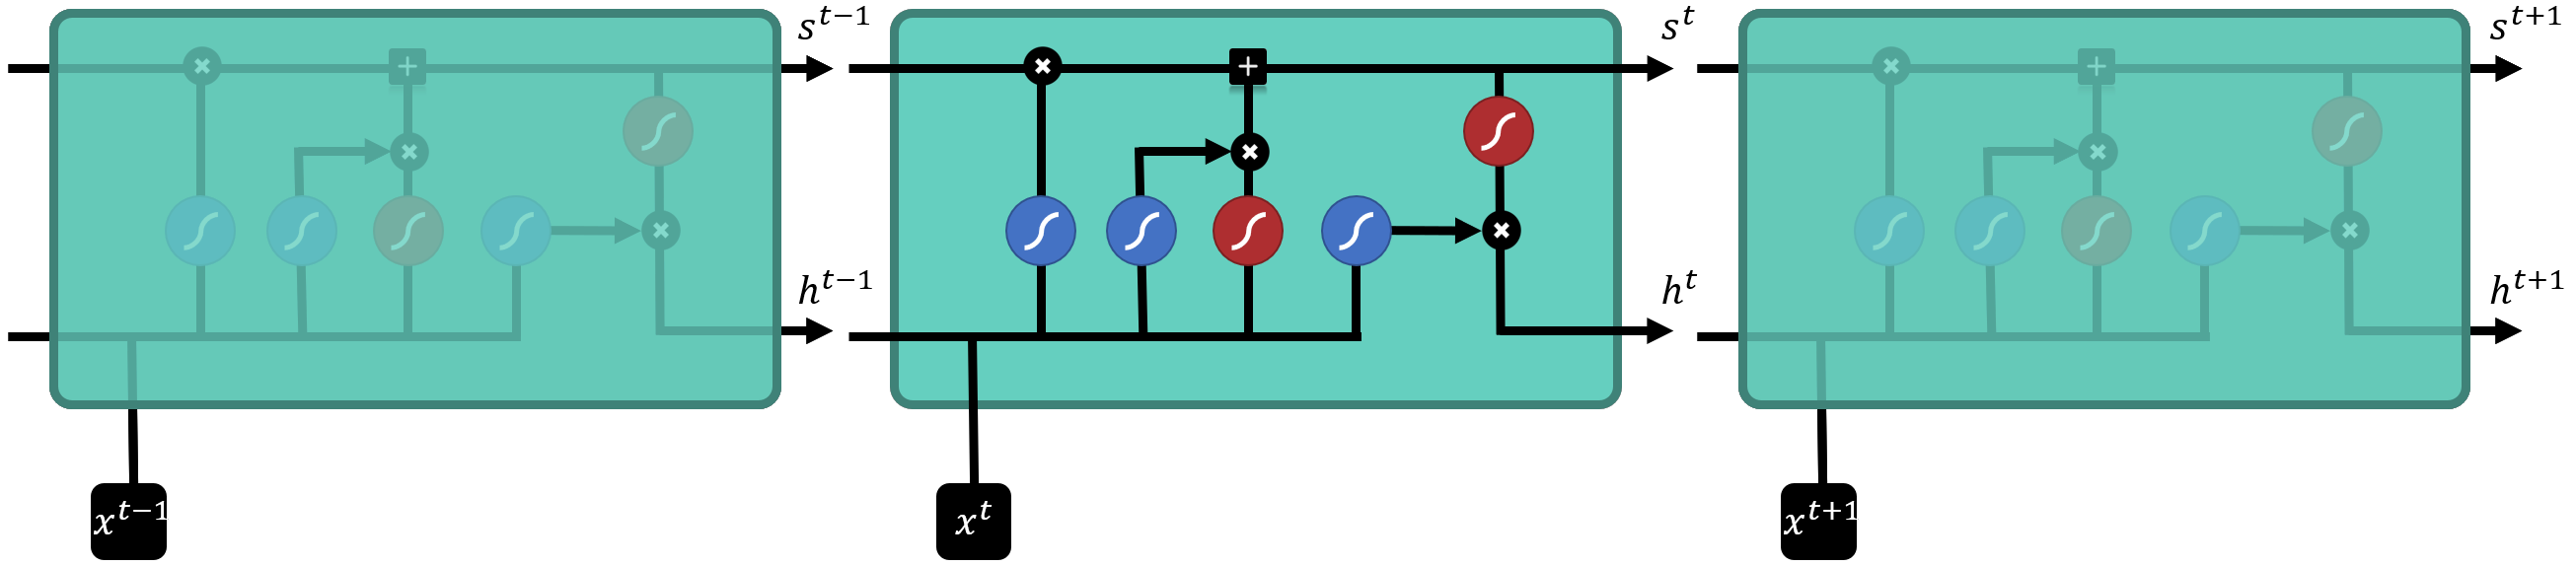
\includegraphics[scale=0.35]{lstm1.png}
    \caption{Срез развернутого LSTM слоя.}
    \label{fig:lstm1}
\end{figure}
Идея вентилей состоит в том, чтобы контролировать вектор значений за счет его умножения на вектор шлюза (вентиля), который управляет потоком ошибки. Целью является сохранение постоянного объема потока ошибки.\\
\begin{figure}[ht]
    \centering
    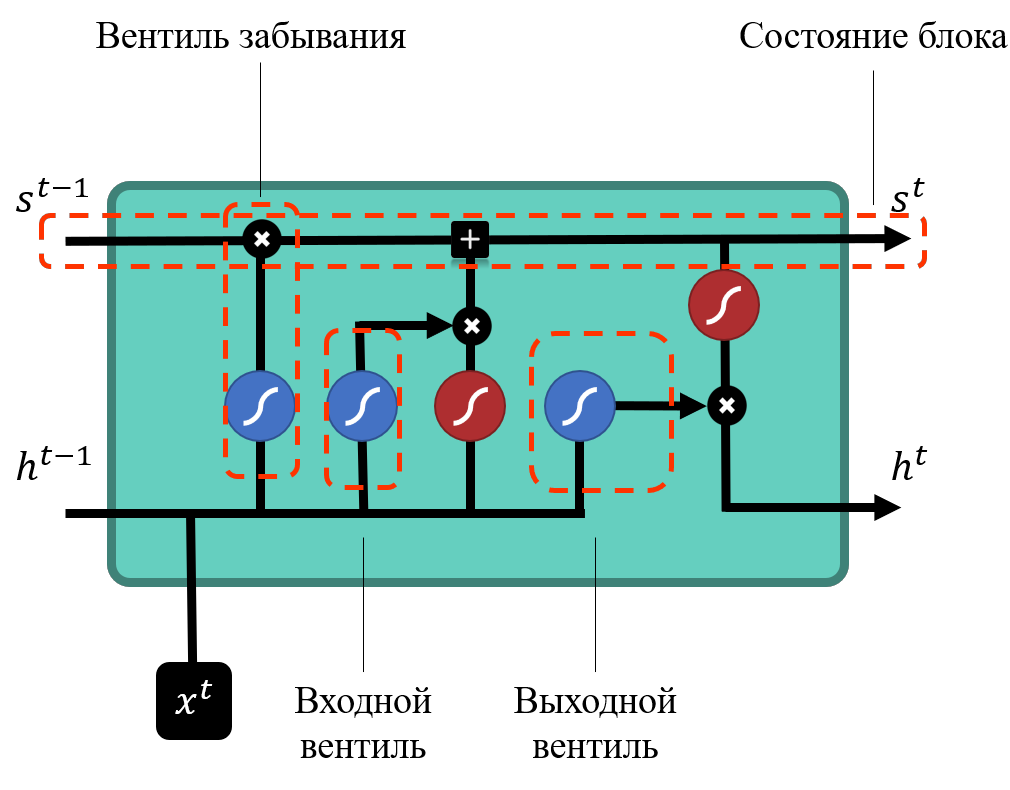
\includegraphics[scale=0.7]{lstm2.png}
    \caption{LSTM блок.}
    \label{fig:lstm2}
\end{figure}

\bigskip\par
Запишем формальный прямой ход LSTM блока в момент времени $t$:
\begin{itemize}
    \item Конкатенируем прошлое скрытое состояние $h^{t-1}$ и входной вектор $x^{t}$. Применяем линейное преобразование и нелинейную функцию активации:
    \begin{gather*}
        f_{t} = \sigma\left(W_{f}\cdot \left[h^{t-1}, x^{t}\right] + b_{f}\right);\\
        i_{t} = \sigma \left(W_{i}\left[h^{t-1}, x^{t}\right] + b_{i}\right);\\
        \tilde{s}^{t} = \mathrm{act}\left(W_{\tilde{s}}\cdot \left[h^{t-1}, x^{t}\right] + b_{\tilde{s}}\right);\\
        o_{t} = \sigma \left(W_{o} \cdot \left[h^{t-1}, x^{t}\right] + b_{o}\right);
    \end{gather*}
    $\mathrm{act}$ -- функция активации (например, $\tanh$);
    \item Получим сигнал как линейную комбинацию:
    \[s^{t} = f_{t} \cdot s^{t-1} + i_{t} \cdot \tilde{s}^{t};\]
    \item Выходим из рекуррентного шага:
    \[h^{t} = o_{t}\cdot \tanh (s^{t}).\]
\end{itemize}
$f_{t}$ -- вентиль забывания (forgetting gate), обучаемый за счет весов $W_{f}$ и сдвига $b_{f}$, определяющий насколько нужно забыть состояние с прошлого блока.\\
$i_{t}$ -- входной вентиль (input gate), обучаемый за счет весов $W_{i}$ и сдвига $b_{i}$, ответственный за чувствительность ко входу: определяет, насколько важно для запоминания полученное новое состояние $\tilde{s}^{t}$. Состояние $\tilde{s}^{t}$ в рекуррентных сетях без вентильной парадигмы было бы выходом блока.\\
$o_{t}$ -- выходной вентиль (output gate), применяемый для увеличения точности аппроксимации нейронной сети за счет нелинейности функции активации.

\bigskip\par
За счет того, что сигмоида принимает значения в диапазоне: $0 < \sigma < 1$, все значения вентилей находятся в этом же диапазоне, что позволяет управлять амплитудой значений состояний, не меняя знак и контролируя объем потока ошибки. \\
Внутренние работы с новыми и старыми состояниями позволяют классифицировать их важность, как следствие настроить запоминание и забывание того, что нужно для решения задачи и бесполезно, соответственно. LSTM достаточно успешно представляет долгосрочные зависимости, моделирует язык, позволяет решать широкий спектр задач, но не лишена проблем. За счет появления новых внутренних обучаемых весов и сдвигов увеличивается количество обучаемых параметров в 4 раза по сравнению с обычной рекуррентной нейронной сетью. Поэтому LSTM часто может переобучаться и показывать плохие результаты на новых данных.
\subsubsection{Управляемый рекуррентный блок (GRU)}
Уменьшить количество обучаемых параметров без сильной потери качества удалось сети GRU (gated recurrent unit, управляемый рекуррентный блок). Основная идея остается той же -- сохранение постоянства объема потока ошибки.
\begin{figure}[H]
    \centering
    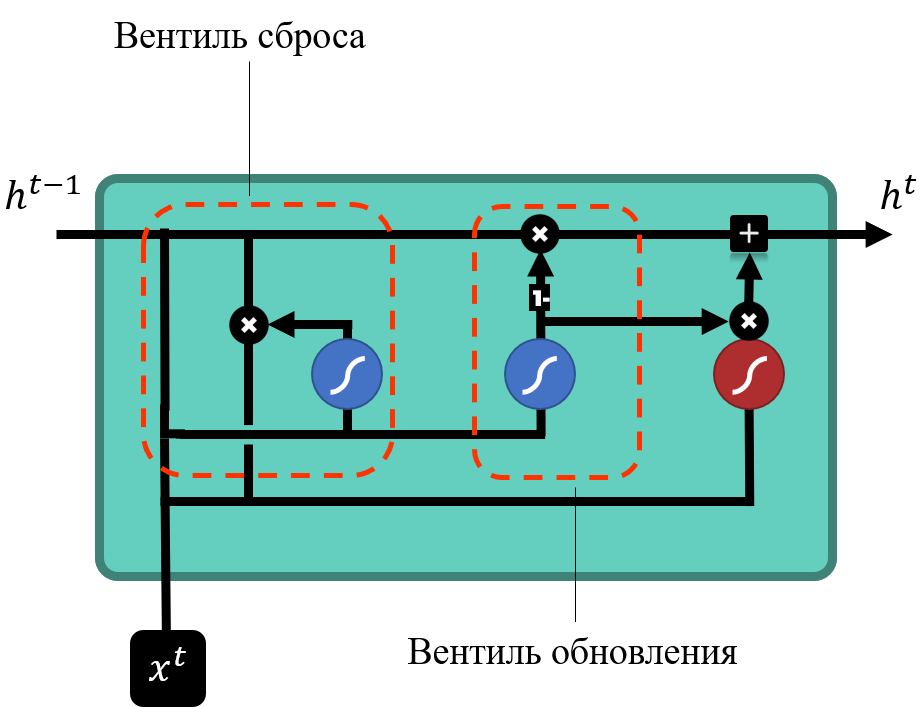
\includegraphics[scale=0.7]{gru1.png}
    \label{gru1}
    \caption{GRU блок}
\end{figure}

\bigskip\par
Запишем формальный прямой ход GRU блока в момент времени $t$:\\
\begin{itemize}
    % \setlength\itemsep{-0.5cm}
    \item Конкатенируем $h^{t-1}$ и $x^{t}$. Применяем линейное преобразование и нелинейную функцию активации:
    \begin{gather*}
        u_{t} = \sigma \left(W_{u} \cdot\left[x^{t}, h^{t-1}\right]\right);\\
        r_{t} = \sigma\left(W_{r} \cdot \left[x^{t}, h^{t-1}\right]\right);\\
        \tilde{h}^{t} = \mathrm{act} \left(W \cdot \left[x^{t}, r_{t} \cdot h^{t-1}\right]\right);
    \end{gather*}
    $\mathrm{act}$ -- нелинейная функция активации (например, $\tanh$);
    \item Получим сигнал как линейную комбинацию:
    \[h^{t} = \left(1 - u_{t}\right)\cdot h^{t-1} + u_{t} \cdot \tilde{h}^{t}\]
    \item Выходим из рекуррентного шага.
\end{itemize}
$u_{t}$ -- вентиль обновления (update gate), решающий на каждом состоянии, оставить предыдущее значение или обновить.\\
$r_{t}$ -- вентиль сброса (reset gate), позволяющий контролировать поведение обновленного состояния. В результате, количество обучаемых параметров сократилось на треть (до порядка $6d^{2}$, где $d$ -- глубина реккурентного слоя). Сеть стала значительно проще в обучении, не потеряв мощности.
\subsubsection{Недостатки и способы борьбы с ними}
Традиционные рекуррентные нейронные сети не подвергаются распараллеливанию вычислений, 
так как происходит последовательная обработка данных. Из-за этого обучение происходит 
ощутимо дольше, чем для других нейронных сетей. Кроме того, из-за умножения большого числа параметров и производных функций активаций при обратном распространении ошибки возникают проблемы взрыва и затухания градиента, подходы для решения которых существуют, однако ухудшающие возможное качество моделей. Целенаправленно для решения этих проблем была разработана архитектура LSTM, которая, следуя парадигме вентильных нейронных сетей, способна контролировать процессы запоминания и забывания последовательной информации, однако, это приводит к значительному увеличению обучаемых параметров. Решению этой проблемы LSTM посвящены архитектуры GRU и Simple-RNN, первая из которых использует концепцию одного вентиля, управляющего обоими процессами, и, на практике показывает схожее с LSTM качество, с ощутимым приростом производительности. Simple-RNN показывает качество хуже, хоть и имеет на треть меньшее количество параметров, чем GRU. Для задачи ВКР Simple-RNN был исключен, однако, не сказать о возможности уменьшения количества обучаемых параметров в рамках повествования о рекуррентных нейронных сетях считаю неправильным.%! описать концепт 
